% U-Net architecture (64 base channels, 256×256×4 NAIP input)
% Compile:  pdflatex unet_architecture.tex
% Requires: tikz, calc, arrows.meta, positioning
%
% Modern block-diagram style — each encoder/decoder level is a labeled box.
% Skip connections are horizontal dashed arrows.

\documentclass[tikz, border=14pt]{standalone}
\usepackage{tikz}
\usetikzlibrary{arrows.meta, positioning, calc}

% ── Colour palette (matches repo figure style) ──────────────────────────────
\definecolor{cenc}{RGB}{59,  120, 196}   % encoder blue
\definecolor{cdec}{RGB}{46,  155,  82}   % decoder green
\definecolor{cbn} {RGB}{123,  79, 166}   % bottleneck purple
\definecolor{cpool}{RGB}{192,  57,  43}  % max-pool red
\definecolor{cup} {RGB}{ 39, 174,  96}   % up-conv green
\definecolor{cskip}{RGB}{230, 126,  34}  % skip / copy orange
\definecolor{cout} {RGB}{127, 140, 141}  % output gray

% ── Reusable node styles ─────────────────────────────────────────────────────
\tikzset{
  enc/.style  = {rectangle, fill=cenc,  draw=white, line width=0.5pt,
                 text=white, font=\small,
                 minimum width=3.2cm, minimum height=0.75cm},
  dec/.style  = {rectangle, fill=cdec,  draw=white, line width=0.5pt,
                 text=white, font=\small,
                 minimum width=3.2cm, minimum height=0.75cm},
  bn/.style   = {rectangle, fill=cbn,   draw=white, line width=0.5pt,
                 text=white, font=\small,
                 minimum width=3.2cm, minimum height=0.75cm},
  outn/.style = {rectangle, fill=cout,  draw=white, line width=0.5pt,
                 text=white, font=\scriptsize,
                 minimum width=0.75cm, minimum height=0.75cm},
  >=Stealth, thick
}

\begin{document}
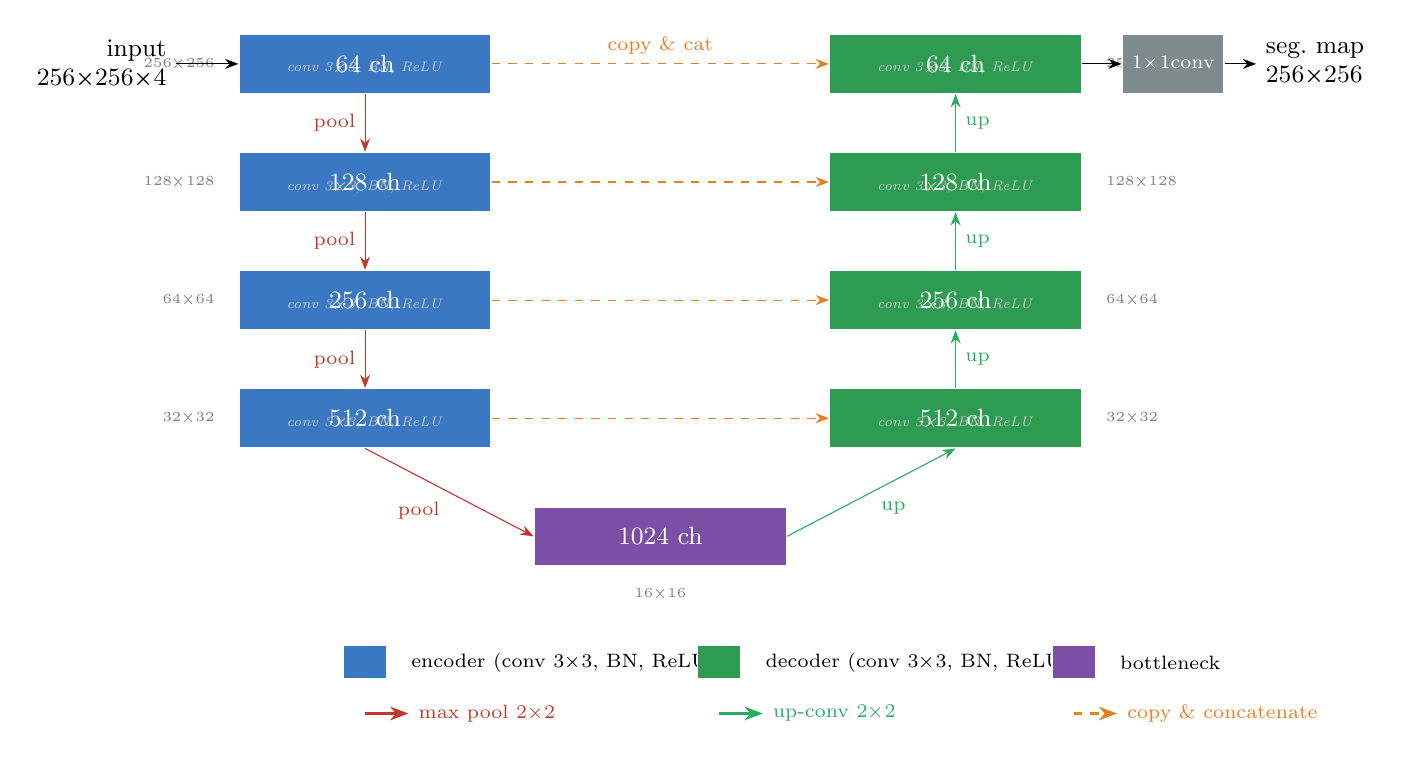
\begin{tikzpicture}

% ── Row y-coordinates (top → bottom) ─────────────────────────────────────
\def\yA{6.0}   % level 0 : 64 ch  / 256×256
\def\yB{4.5}   % level 1 : 128 ch / 128×128
\def\yC{3.0}   % level 2 : 256 ch /  64×64
\def\yD{1.5}   % level 3 : 512 ch /  32×32
\def\yBN{0.0}  % bottleneck : 1024 ch / 16×16

% Encoder x  |  Decoder x
\def\xE{0.0}
\def\xD{7.5}

% ── Encoder blocks ─────────────────────────────────────────────────────────
\node[enc] (e0) at (\xE, \yA)  {64 ch};
\node[enc] (e1) at (\xE, \yB)  {128 ch};
\node[enc] (e2) at (\xE, \yC)  {256 ch};
\node[enc] (e3) at (\xE, \yD)  {512 ch};

% ── Bottleneck ─────────────────────────────────────────────────────────────
\node[bn]  (bn) at (3.75, \yBN) {1024 ch};

% ── Decoder blocks ─────────────────────────────────────────────────────────
\node[dec] (d3) at (\xD, \yD)  {512 ch};
\node[dec] (d2) at (\xD, \yC)  {256 ch};
\node[dec] (d1) at (\xD, \yB)  {128 ch};
\node[dec] (d0) at (\xD, \yA)  {64 ch};

% ── Spatial-size labels (outside the blocks) ────────────────────────────────
\foreach \n/\sp in {e0/256, e1/128, e2/64, e3/32}
  \node[font=\tiny, gray, left=0.18cm of \n] {\sp×\sp};
\node[font=\tiny, gray, below=0.15cm of bn] {16×16};
\foreach \n/\sp in {d3/32, d2/64, d1/128, d0/256}
  \node[font=\tiny, gray, right=0.18cm of \n] {\sp×\sp};

% ── Encoder downsampling arrows ─────────────────────────────────────────────
\draw[->, cpool] (e0.south) -- node[left,  font=\scriptsize, cpool] {pool}  (e1.north);
\draw[->, cpool] (e1.south) -- node[left,  font=\scriptsize, cpool] {pool}  (e2.north);
\draw[->, cpool] (e2.south) -- node[left,  font=\scriptsize, cpool] {pool}  (e3.north);
\draw[->, cpool] (e3.south) -- node[below left, font=\scriptsize, cpool] {pool} (bn.west);

% ── Decoder upsampling arrows ───────────────────────────────────────────────
\draw[->, cup]   (bn.east)  -- node[below right, font=\scriptsize, cup] {up}  (d3.south);
\draw[->, cup]   (d3.north) -- node[right, font=\scriptsize, cup] {up}        (d2.south);
\draw[->, cup]   (d2.north) -- node[right, font=\scriptsize, cup] {up}        (d1.south);
\draw[->, cup]   (d1.north) -- node[right, font=\scriptsize, cup] {up}        (d0.south);

% ── Skip connections (copy & concatenate) ──────────────────────────────────
\draw[->, cskip, dashed]
  (e0.east) -- node[above, font=\scriptsize, text=cskip] {copy \& cat} (d0.west);
\draw[->, cskip, dashed] (e1.east) -- (d1.west);
\draw[->, cskip, dashed] (e2.east) -- (d2.west);
\draw[->, cskip, dashed] (e3.east) -- (d3.west);

% ── Input arrow ─────────────────────────────────────────────────────────────
\draw[->] (-2.4, \yA) -- (e0.west)
  node[pos=0.0, left,  font=\small] {\shortstack[r]{input\\256×256×4}}
  node[pos=0.55, above, font=\scriptsize, gray] {};

% ── Output: 1×1 conv → prediction ───────────────────────────────────────────
\node[outn, right=0.5cm of d0] (out) {1×1\\conv};
\node[right=0.4cm of out, font=\small] (pred) {\shortstack[l]{seg.\ map\\256×256}};
\draw[->] (d0.east)  -- (out.west);
\draw[->] (out.east) -- (pred.west);

% ── "conv 3×3, BN, ReLU" sub-labels inside each block ───────────────────────
\foreach \n in {e0,e1,e2,e3,d0,d1,d2,d3}
  \node[font=\tiny, gray!40!white, below=0pt of \n.center, yshift=4pt]
        {\textit{conv 3×3, BN, ReLU}};

% ── Legend ──────────────────────────────────────────────────────────────────
\begin{scope}[shift={(0.0, -1.6)}]
  % Row 1
  \node[enc, minimum width=0.55cm, minimum height=0.42cm] (le) at (0, 0) {};
  \node[right=0.18cm of le, font=\scriptsize] {encoder (conv 3×3, BN, ReLU)};

  \node[dec, minimum width=0.55cm, minimum height=0.42cm] (ld) at (4.5, 0) {};
  \node[right=0.18cm of ld, font=\scriptsize] {decoder (conv 3×3, BN, ReLU)};

  \node[bn,  minimum width=0.55cm, minimum height=0.42cm] (lb) at (9.0, 0) {};
  \node[right=0.18cm of lb, font=\scriptsize] {bottleneck};

  % Row 2
  \draw[->, cpool, thick] (0, -0.65) -- ++(0.55, 0)
    node[right, font=\scriptsize] {max pool 2×2};
  \draw[->, cup,   thick] (4.5, -0.65) -- ++(0.55, 0)
    node[right, font=\scriptsize] {up-conv 2×2};
  \draw[->, cskip, dashed, thick] (9.0, -0.65) -- ++(0.55, 0)
    node[right, font=\scriptsize] {copy \& concatenate};
\end{scope}

\end{tikzpicture}
\end{document}
